\section{Thesis Progress \& Plan}

\begin{frame}{Work So Far}
	Thus far, most of the work on my thesis has been split between three tasks:
	
	\begin{enumerate}
		\item Familiarising with one particular implementation: JIF (Java Information Flow)
		\item Researching information flow models and implementations
		\item Researching the applicability of information flow to real security problems
	\end{enumerate}
\end{frame}

\begin{frame}{JIF}
	Java Information Flow is a language extension to Java with `mostly static' information flow features through `security types', which are policies as per the Decentralised Label Model \cite{work:myersdlm}.
	
	Every variable has a security label attached to it which encodes how its information may flow between principals. For instance:
	
	\texttt{int\{Alice->Bob\} x;}
	
	indicates that principal Alice owns the information, and allows that information to flow to Bob or a principal Bob has delegated authority to.
\end{frame}

\begin{frame}{JIF: A Minimal `Hello World'}
	\begin{figure}
		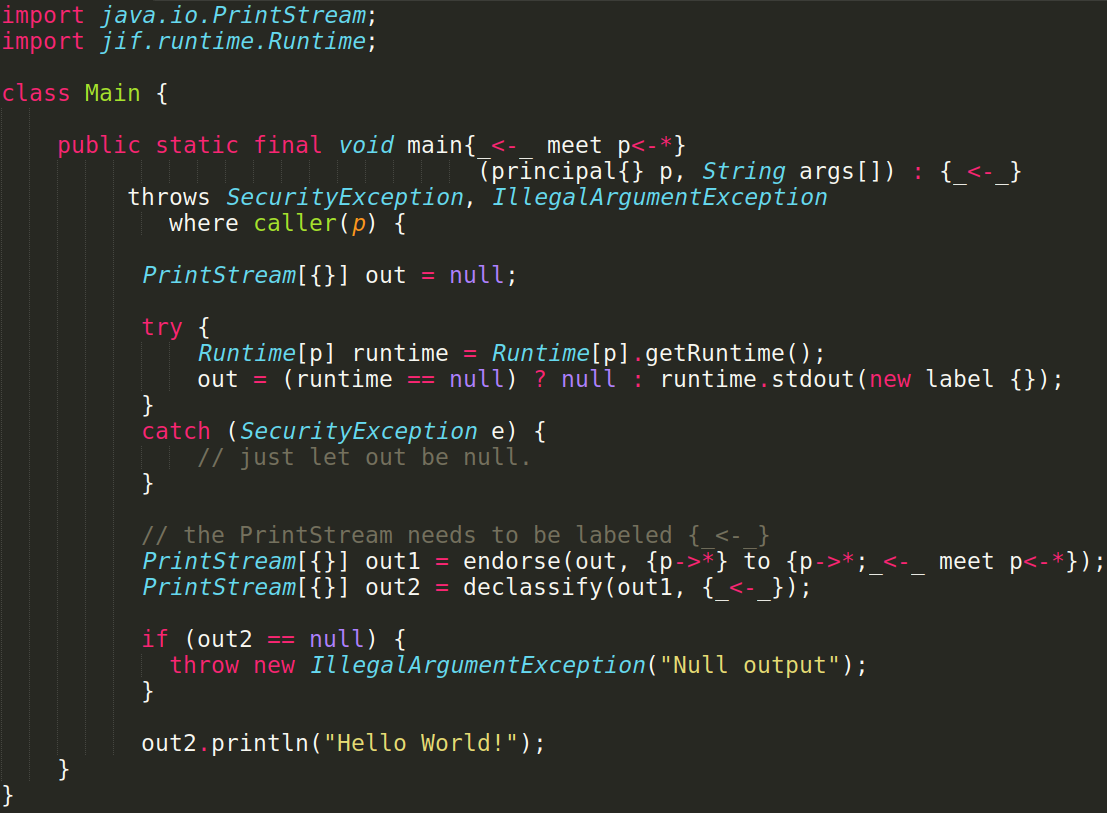
\includegraphics[width=\linewidth]{content/images/jif_helloworld.png}
	\end{figure}
\end{frame}

\begin{frame}{JIF: Static Checking Errors}
	\begin{figure}
		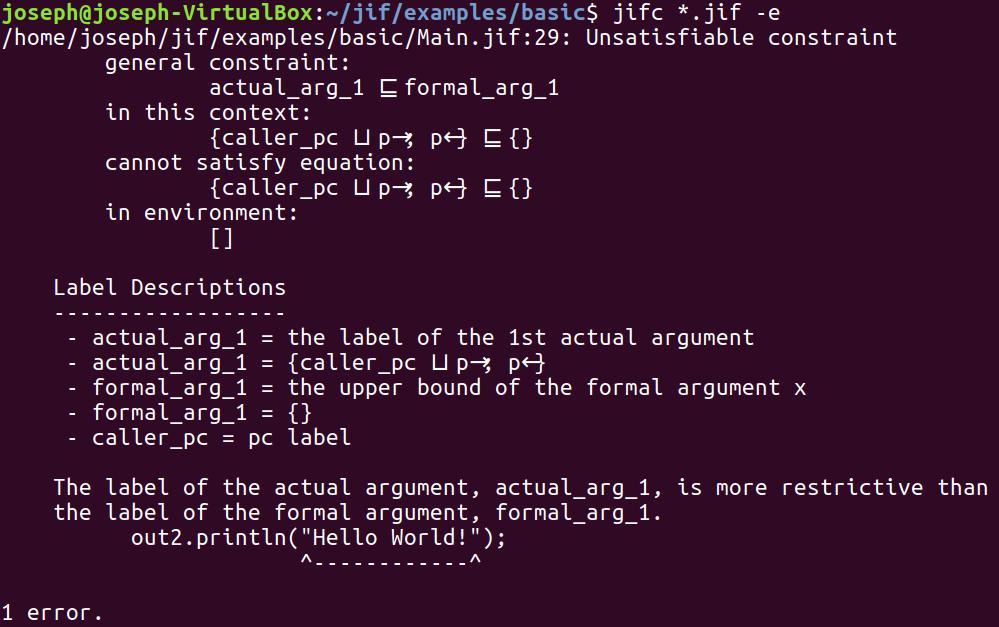
\includegraphics[scale=0.5]{content/images/jif_helloworld_error.png}
		\caption{A JIF compiler error}
	\end{figure}
\end{frame}

\begin{frame}{JIF: Practicality \& Programmer Burden}
	
	JIF's issues:
	
	\begin{itemize}
		\item Inherently complex policies
		\item Programmer burden compounds as complexity increases
		\item Sparse documentation, no debugger, misleading compiler errors
		\item Interoperability issues with Java
	\end{itemize}
	
	\note{
		Thus far in my research, JIF's largest problem has proven to be the complexity of its policies and the programmer burden that induces.
		
		JIF inherently places a large cognitive burden on the programmer: the programmer must provide correct policies for flows within the system at every level, which compounds as programs get larger, and as they have to perform more complex tasks, which makes writing modular programs difficult.
		
		While documentation is sparse, and the compiler's error messages often do not correspond to the true information flow problem, these merely exacerbate the core burden issue.
		
		In addition, though Jif has the advantage of being based on Java, interoperability is limited -- features like reflection do not exist, and external libraries require JIF signatures for their interfaces.
		}
	
	
\end{frame}

\begin{frame}{LIFTy -- An Alternate Approach}
	LIFTy is a different information flow-secure language, that provides some solutions to these problems. Specifically, code is \textbf{policy agnostic}, and the policies are simple predicates rather than complex DLM labels.
	
	LIFTy is not Java-based; it is a statically typed $ \lambda $-calculus based language that uses `type driven program repair' to automatically add access checks on confidential data during compilation.
\end{frame}

\begin{frame}{Other Implementations}
	\begin{enumerate}
		\item Paragon
		\item LIFTy
		\item Dynamic ones
	\end{enumerate}
\end{frame}

\begin{frame}{General Applicability}
	Oracle Guidelines
	
	Untrusted code vs Untrusted data
	
	Actual exploits
\end{frame}

\begin{frame}{Overall Thoughts}
	`Heavy' programmer burden
	
	Not relevant for most security issues
	
	Potential for `lighter' solutions (e.g. LIFTy, static analysis tools)
\end{frame}